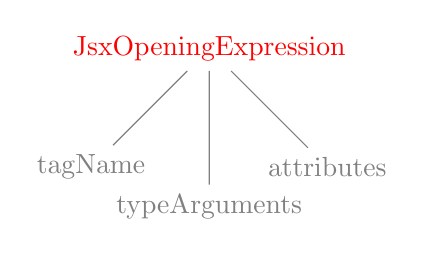
\begin{tikzpicture}
	\node [red] {JsxOpeningExpression}
		child [gray] {node [gray] {tagName}}
		child [gray] {node [gray, yshift = -0.5cm] {typeArguments}}
		child [gray] {node [gray] {attributes}};
\end{tikzpicture}
\caption[LoF entry]{
	Node pattern for a JSX opening element (as supported in React\footnote{\url{https://reactjs.org/docs/introducing-jsx.html}} or TypeScript\footnote{\url{https://www.typescriptlang.org/docs/handbook/jsx.html}}), such as in:
	\code{\lowlight{elem = }\uline{<Button \lowlight{color}="\lowlight{blue}"> \lowlight{Google</Button>}}\lowlight{;}}
}
